% Chapter Template

\chapter{Nucleosynthesis} % Main chapter title

\label{ChapterX} % Change X to a consecutive number; for referencing this chapter elsewhere, use \ref{ChapterX}
%% =======================================================
%%
%%                   Nucleosynthesis
%%
%% =======================================================

\textcolor{red}{Based on the Jones Lippuner PhD thesis}

For a long time the general consensus was that all elements in the universe were synthesized during the Big Bang \citep{Alpher:1948}. Later studies have, however, proven that only elements with atomic number $A<8$ were produced (see \textit{e.g.,} \citet{Alpher:1950,Shaviv:2012}). Thus, only the lightest elements, hydrogen and helium primarily, were produced during in the Big Band \citep{Burbidge:1957}. Heavier elements are synthesized in a plethora of processes that we briefly recall here.

In this chapter we discuss the rapid neutron capture process (\rproc{}) responsible for creation of heavy elements \cite{Burbidge:1957}. We introduce conditions and cites of \rproc{}, its contribution to the Universe' chemical evolution. We briefly discuss how numerous nuclear species, participating in thousands on nuclear reactions, are evolved using the novel \texttt{SkyNet} nuclear reaction network code. Then, we consider binary neutron star mergers as a source of \rproc{} elements. We compute the nucleosynthetic yields from mergers, using the \ac{NR} \ac{BNS} simulations performed with \texttt{WhiskyTHC} code (see sec. \ref{sec:code:WhiskyTHC}) and analyzed in Sec.\ref{sec:ejecta:results}.



\section{Introduction}

It is of paramount importance for testing nucleosynthesis theories and models to have an accurate measurements of relative abundances in the Universe. For Humanity, confined still to just one planet, this is not a trivial task. And while automatic spacecrafts, such as Luna, Apollo and Hayabusa have delivered samples from asteroids, most of the studies are performed using the naturally falling meteorites. The composition of these guests from space is then thoroughly studied via absorption and emission spectroscopy \citep{Shaviv:2012}.

The understanding of the solar system isotope and element abundances  have come a long way \citep[\eg][]{Cameron:1973,Anders:1989,Grevesse:1998,Lodders:2003} 
\textcolor{red}{add last papper you used for solar A.}

%% \begin{sidenote}
%%     \textcolor{red}{Figure with solar observed abundances, showing $r$-elements and $s$-elements}
%%     The observed obundacnes as a function of atomic mass number $A$ are shown in figure Fig. (XXX). (data from \cite{Lodders:2003}). The plot shows nuclei that are more bound (due to spin pairing of nucleons \cite{Moller:1993ed}), \textit{i.e,} those with an even $A$ number, are more abundant. The lowest binding energy of nuclei with odd number of neutrons and protons (but even $A$) are largely unstable or short-lived. A few exceptions are \textit{e.g.,} $^{40}$K, $^{50}$V, $^{138}$La and $^{176}$Lu, that have a half-life of at least $10^{9}$ years.
%% \end{sidenote}

The dominant \nuc{} process, responsible for the production of elements, varies with the mass range.

For instance, light elements $A<8$ were synthesized right after the Big Bang. Nuclides before the iron peak, $12\leq A\leq 56$ come from stellar hydrostatic nuclear burning, elements at the iron peak $50\leq A \leq 62$ produces mostly during the type Ia \acp{SN} or explosive silicon burning in \acp{CCSN}. The conditions at these sights are such that the dense material at the \ac{NSE}, expands and cools down. Most of the material beyond iron peak are produced via neutron capture processes \cite{Burbidge:1957}.


%% =======================================================
%%
%%                   Nucleosynthesis Cites
%%
%% =======================================================

\subsection{Nucleosynthesis up to the iron peak}


\subsubsection{Big Bang nucleosynthesis}

Light elements in the Universe, like hydrogen ($\sim 75\%$ by mass) and helium ($\sim 25\%$ by mass) alongside trace amounts of $^{3}$He and $^{7}$Li were created during the \ac{BBN} (see \eg, \citet{Tytler:2000qf} and references therein). And while only a small number of nuclides were involved in \ac{BBN}, there are large discrepancies between \ac{BBN} models and observations. For instance, the "lithium problem" \citep{Coc:2013eha}, which origin is not well understood \citep{Fields:2011zzb}.


\subsubsection{Low-mass stellar burning}

In order to fuse massive nuclides and overcome the strong Coulomb barrier, high temperatures, ($\geq 10^6$ K) are required. Thus production of heavy elements from hydrogen and helium is possible only in special environments, in particular, in the interior of stars \citep{Bethe:1939}. 
For the most of their lives stars burn hydrogen into helium. The process releases the binding energy and maintains the hydrostatic stability of a star. After the hydrogen is exhausted in the core, a core (atmosphere) contracts (expands), heats up (cools), and the shell hydrogen burning is initiated, slowly depositing ashes, \eg, helium, into the inert core. 
The star's subsequent evolution depends primarily on its mass. If the mass of a star $M>0.5M_{\odot}$, at some point the helium in the core starts to fuse into $^{12}$C and $^{16}$O and small amounts of $^{24}$Mg, $^{28}$Si. These elements are called \textit{alpha elements} \citep{Rolfs:1988,Hasen:2004}. 
The end of the core helium burning phase leads to another core contraction phase. A star of a mass $\sim 8M_{\odot}$ would be able to ignite carbon and oxygen producing heavier elements afterwards. A less massive star looses its outer layers and becomes a slowly cooling degenerate core, a white dwarf.


\subsubsection{nuclear burning is massive stars}

For a star that has $M\geq 8M_{\odot}$, a sequence of burning stages follows, each of which leads to the exhaustion of a respective fuel, contraction of the core and rise of its temperature \citep{Woosley:2002}. Carbon burning leads to the production of $^{20}Ne$, $^{23}$Na and free protons that contribute to the synthesis of non-alpha elements. As temperature increases, the photodisintegration of $^{20}$Ne becomes possible and a small amount of $^{24}$Mg is formed. Next, the oxygen burning occurs producing $^{28}$Si $^{31}$P, and $^{28}$Si and $^{32}$S, that become dominant nuclides in the core by the end of oxygen burning \citep{Rolfs:1988}.

The subsequent silicon burning proceeds at $T\sim3.5\times10^9$K through photodissociation of some of the $^{28}$Si and a sequence of alpha particle captures, "alpha ladder", on the remaining $^{28}$Si to form $^{32}$S, $^{36}$Ar, $^{40}$Ca, $^{44}$Ti, $^{48}$Cr, $^{52}$Fe and $^{56}$Ni. This process lasts around a day \citep{Rolfs:1988,Hasen:2004}. Due to high temperatures present at silicon burning, nuclides with $A\in[28, 62]$ fall into quasi-equilibrium, meaning that these nuclides (with exception of $^{12}$C, $^{16}$O $^{20}$Ne and $^{24}$Mg), alpha particles and protons participating in reactions, are in equilibrium with each other. 

At $A=56$ the binding energy per nucleon appears reaches its maximum and the silicon burning cannot produce heavier nuclides with the release of energy. As the fraction of $^{56}$Ni in the core of a star increases, the support that nuclear burning has provided against gravitational contraction falls. Meanwhile the mass of the degenerate core still increases as burning proceed in shells. However, when the electron degeneracy pressure can no longer counteract gravity, \ie, when mass of the core exceeds the effective Chandrasekhar mass \footnote{The collapse however occur before the core reaches Chandrasekhar mass, and the pressure support that rests on the availability of free electrons drops when electrons capture on the nuclides becomes possible. To account for this, the effective Chandrasekhar mass was introduced.}, the core collapses leading to a \ac{CCSN} \cite{Woosley:2002}.

Thus, the origin of more abundant alpha elements in the Universe is stellar fusion.


\subsubsection{Iron Peak}

At temperatures higher then $T\sim 5\times10^{9}$K nuclear \ac{NSE} establishes. This is a balance between the fusion reactions forming a ($N,Z$) nuclide from $N$ neutrons and $Z$ protons and photodissociation reactions, splitting it back. At \ac{NSE} three parameters describe the composition: 
%% [IMPORTANT]
density, temperature and electron fraction $Y_e = n_p/(n_p + n_e)$, where $n_e$ and $n_p$ are the (total) 
%% ---
number density of electrons and protons respectively \citep{Seitenzahl:2009}. 

The composition at \ac{NSE} favors more tightly bound nuclides, as they are more difficult to photodissociate. Thus, if the conditions allow, \textit{i.e.,} temperature, density and electron fraction of the mater, ($Y_e \sim 0.46$, an electron fraction of iron), nuclides at $A\sim56$, \textit{i.e.,} iron peak elements, dominate \citep{Seitenzahl:2009}. 

For example, \ac{NSE} establishes during the type Ia \acp{SN}, when a thermonuclear explosion of a white dwarf allows for sufficiently high temperatures and densities. After the explosion, newly synthesized elements of the iron peak cools, and being stable, remain in the expanding medium \citep{Iwamoto:2000as}.


\subsubsection{Nucleosynthesis beyond the iron peak}

Nuclides with $A\geq 56$ cannot be synthesized via standard cycles due to their strong Coulomb barriers. Thus, processes that do not involve charged particles become dominant. These are the neutron capture processes.

As nuclides absorb neutrons and grow larger, their binding energy $Q_n$ decreases. This process is stopped when $Q_n\sim1$~MeV and energetic photons start to knock out neutrons from a nucleus. This process is called photodisintegration and a location in the parameter space where it occurs, (that in turn dependents on temperature and density), is called the 
%% [IMPORTANT]
neutron drip line 
%% ---
\cite{Rolfs:1988}.

Nuclides produced via neutron capture are generally unstable to a $\beta$-decay, with a timescale $\tau_{\beta}$, that can be larger or smaller than a neutron capture timescale, $\tau_n$. 
In case when $\tau_{\beta}\ll\tau_n$, \ie, when a $\beta$-decay occurs faster then the next neutron capture, the process is called \textit{slow} or \sproc{}. 
Thus, by definition, the \sproc{} moves along the valley of stability\footnote{a region of stable nuclides in the nuclides chart, a chart in terms of number of neutrons $n_n$ and number of protons $n_p$.}, departing no further than by a few nuclides away.
On the other hand, if $\tau_{\beta}\gg\tau_n$, \ie, when a neutron capture occurs much faster then a $\beta$-decay, the process is called \textit{rapid} or \rproc{}. This \nuc{} generates nuclides near (but not crossing) the neutron drip line \textcolor{red}{Here a plot, Fig.1.6 from Source would have been useful.} \citep{Rolfs:1988}. 

%% --- IMPORTANT --- ORIGIN OF THE PEAKS IN r-PROCESS
Notably, the trajectory of $r$-process is interrupted when the neutrons within a nuclide can arrange themselves in a closed shell. Such configurations are energetically very favorable and thus the cross section for a subsequent neutron capture reduces. Only after several $\beta$-decays does the $r$-process continue. Thus, nuclides located at points where neutron drip line and closed neutron shell overlap is more abundant. These unstable nuclides will decay back to the valley of stability and some of the neutrons within them turn to protons, reducing the total mass of them. The indication of this "overproduction" are the peaks in the abundance patterns at a mass, $A$, slightly lower then the one corresponding to a closed shell nuclide. \textcolor{red}{here a ref to a fig with Abundances is needed. }. \red{[NEED a FIGURE]} 

%% --- important
A similar "overproduction" of nuclides with a closed neutron shell occurs when an $s$-process is considered. However, in that case it is caused by the cross section of these nuclides being $1-2$ order of magnitude smaller then of neighboring ones \citep{Rolfs:1988}. Thus, in the case of \sproc{}, the peaks in abundance pattern will be at $A$, corresponding to the closed shell exactly, and thus located at larger $A$ than that of the \rproc{}. 
Closed shell nuclides are located at $N=50,\: 82, \: 126$ and thus corresponding abundance peaks for $s$-process are at $A=88, \: 138, \: 208$ and at $A=80,\:130,\:194$ for $r$-process (see \textit{e.g.,} \citet{Arnould:2007gh}) 
\textcolor{red}{abundance peaks with 'r' and 's' elements is needed.}

%% --- Motivation MP stars --- THE GENERIC SOLAR ABUNDANCES
It was found, that the solar $r$-process abundance pattern of \rproc{} is consistent, and can be found anywhere in the Universe. In particular, in stars that were formed very early on a galactic evolution timescale, the metal poor halo stars, one would expect to observe less \sproc{} and \rproc{} elements as there might have been not enough time for the enrichment to take place. However recent studies showed that the solar \rproc{} abundances are present in these stars as well \cite{Sneden:2008,Roederer:2010}, see also Fig.~$8$ in \cite{Sneden:2009} \textcolor{red}{and section 1.9}. Thus, modeling the \rproc{} \nuc{} it is expected to reproduce the solar abundances. \textcolor{red}{once again, a figure can be good}

%% -- can be deleted
It is important to note that in addition to \sproc{} and \rproc{}, a possible $i$-process, (intermediate) is widely discussed. The process operates further from the valley of stability than \sproc{}, but not reaching neutron drip line \citep{Cowan:1977,Bertolli:2013gka}. Slow and intermediate neutron capture processes operate within the low-mass \ac{AGB} stars with mass $M\in[1.5,3]M_{\odot}$ and more massive stars, that enrich the interstellar medium with heavy elements via strong winds  \citep[\eg][]{Peters:1968,Couch:1974,Kaeppeler:1994K,Woosley:2002,Straniero:2005hc,Herwig:2011}. The possible cites for the \rproc{} we discuss in the following subsections.


\subsubsection{Possible \rproc{} sites}

Study of possible cites of \rproc{} is a wide and rapidly developing field. 
The general requirement for \rproc{} is a low electron fraction, or, in other words, neutron-rich conditions. These can be found in a various places for certain models of Big Bang, that include inhomogeneities, \ac{BNS} and \ac{NSBH} mergers and supernova ejecta (see \cite{Mathews:1990} and references therein). Spectral study of \ac{MP} stars, combined with models of galactic chemical evolution sheds light on possible dominant cite of \rproc{} material. \textcolor{red}{add more sources/models}. It is now believed that certain types of \acp{SN} and \ac{BNS} mergers are the most likely sources on \rproc{} material \citep{Mathews:1990,Thielemann:2011} \textcolor{red}{add more sources}


\paragraph{\acp{CCSN}}

Collapse of a massive star produces a hot neutron core, that undergoes deleptonization, releasing $\sim10^{53}$~erg of binding energy in form of strong neutrino flux. These neutrinos, irradiating dense medium around the core, can produce a \nwind{} \citep{Qian:1996xt}, that was suggested to be a promising cite for \rproc{} \citep{Woosley:2002,Wanajo:2006mq}. Later, it was shown however, that the electron fraction in the wind would be too high for a full \rproc{}, and only "light" heavy nuclide up to $A\sim130$ can be synthesized \citep{Qian:1996xt,Thompson:2001ys,Fischer:2010,Roberts:2010,MartinezPinedo:2012rb,Wanajo:2013} \textcolor{red}{add Perego:2017} 

It is important to note, in the proton-rich \nwind{} nuclides with $A\sim 100$ can be produces via so-called $\nu p$-process. The process relies on a creation of a free neutron from proton by an antineutrino capture. This free neutron can then be captured by a seed nuclide, $^{64}$Ge seed nuclide and thus nuclides heavier then $^{64}$Ge can be created \citep{Frohlich:2006,Pruet:2005qd,Wanajo:2010mc,Arcones:2012}

A full \rproc{} can be achieved in so-called magnetorotationally driven \acp{CCSN}. This is a rare type of \acp{CCSN}, where a core of a progenitor is rotating rapidly and strongly magnetized. Induced by a magnetorotational processes \eg, magnetorotational instability, collapse is accompanied by a formation of a collocated bipolar jet \citep{Wheeler:2000,Akiyama:2003,Burrows:2007yx,Mosta:2014jaa,Mosta:2015} \textcolor{red}{add Siegel2019?.}. Materiel in these jets is predicted to be sufficiently neutron rich to allow for a full \rproc{} nucleosynthesis \citep{Winteler:2012,Nishimura:2015nca}. The rarity of this type of \acp{SN}, however, might not allow it to be the dominant source or $r$-process material \cite{Nishimura:2015nca} (\red{See however Seigal:PAPER}). 


\paragraph{\ac{BNS} mergers}
\red{TO BE REWRITTEN -- REPETITION OF PREVIOUS CHAPTERS}

%% --- MIGHT NEED TO BE SHORTENED A LOT!  OR MOVED TO INTRODUCTION!
Mergers of two \acp{NS} or a \ac{NS} and a \ac{BH} are regarded as one of the main cites of \rproc{} material. Formed in a evolution of a binary of massive stars, compact objects orbit each other for gigayears, before slow loss of energy from the system due to gravitational waves reduces their orbit and they merge \citep{Hulse:1975,Lattimer:2004sa,Price:2006fi}. 

The late inspiral and merger of \ac{BNS} or a \ac{NSBH} have been studied extensively via smooth particle simulations \red{[REFS]} \ac{HD} simulations \red{[REFS]} and \ac{NR} simulations with simplified gravity \red{[REFS]} or full \ac{GR} \red{[REFS]}. The composition of a \acp{NS} in these simulations have been modeled with simplified polytropic \red{[REFS]} or piece-wise polytropic \red{[REFS]} or microphsyical \acp{EOS} \red{[REFS]}. The physical setup of these simulations have also evolved to eventually include effects of neutrino radiation transport \red{[REFS]} and magnetic fields \red{[REFS]}. 

These studies have shown that shortly before and during the merger, the neutron star(s) undergo(s) a tidal deformation and disruption. Streams of neutron-reach matter are then ejected into the circombinary with enough energy to be not graviationally bound to the system \citep{Price:2006fi,Foucart:2014nda,Sekiguchi:2015dma,Kyutoku:2015gda,Radice:2016dwd}. 

For details on the ejecta from \ac{BNS} mergers see Chapter \ref{ch:BNS_results}.
%% In addition, in case of a \ac{BNS}, when \acp{NS} collide, material at the collision interface, heated by shocks, gets 'squeezed' and launched in the directions perpendicular to the plane of the binary \cite{Bauswein:2013,Hotokezaka:2013b} \red{[REFS]}. 
%% Generally, these tow components, tidal and shocked, constitute the \textit{dynamical ejecta}. Where the term ejecta referrers to the material that has enough energy to leave the system. 
%% The properties of the dynamical ejecta from BNS have a broad distribution, especailly in terms of mass and ejectron fraction [\red{[REFS]} \& myFitPaper], where the former lies in range $(10^{-4},10^{-2})M_{\odot}$ and the latter $(0.05,0.45)$. We discuss dynamical ejecta properties of BNS in more details in section \red{sec:results:dyn\_ej:prop} and nucleosynthesis in it in \red{sec:results:dyn\_ej:nucleo}. In case of NSBH the ejecta mass was shown be larger, reaching $0.1M_{\odot}$ with low electron fraction, $\leq0.2$ but it requires that masses of BH and NS are comparable and BH is rapidly spinning \cite{Foucart:2014nda}\red{[REFS]}. If the BH is much more massive then NS, the latter would be 'swallowed' with no ejecta \red{[REFS]}.
%% After the merger, there are expected to be additional ejecta. For general postmerger configuration consists of a remnant, massive neutron star (MNS) or a black hole sorrounded by a disk (torus) of bounded matter. In the first case,  a strong neutrino flux from cooling MNS and disk can drive an outflow in the direction, perpendicular to the plane of the binary, the so-called \textit{neutrino-driven wind} (see Figure 1 from \cite{Perego:2014fma}) \red{[REFS],Jujibayashi+20}. This ejecta is expected to occure on a timescales of $\sim100$ms postmerger, be not very neutron rich $Y_e\sim(0.2-0.45)$ due to neutrino irradiation and have a mass of $(10^{-4}-10^{-3})M_{\odot}$ \red{[REFS]}. 
%% The massive nutron star born in a merger exhibit dynamical oscillations \red{[REFS]}. The $m=1$ mode, so-called "one-armed spiral instability" especially can persisit on a $\sim100$ms powtmerger timescale and become a dominant mode \red{[REFS], MainPaper}. This oscillations can inject energy within the disk, where via angular momentum transport it leads to an outer part of the disk to become unbound. This ejecta, the \textit{\swind{}} was shown to occur in all cases where the MNS is present. It has high electron fraction and its mass depends on a lifetime of the remnant, and for a $\sim100$ms it can amount to a few $\times\sim10^{-2}M_{\odot}$ \red{[Letter, MainPaper]}. We discuss the mechanism that drives the \swind{} in the section \red{sec:results:swind:mechanism} and the ejecta properties in \red{sec:results:swind:prop} and corresponding nucleosynthesis in \red{sec:results:swind:nucleo}.
%% On a longer timescales, the viscous processes and alpha recombination in the disk, surrounding MNS or a BH are expected to unbind additional material. This is so-called \textit{secular ejecta}. It is expected to be massive and neutron rich. However, due to long timescales involved, it is very difficult model \red{[REFS]}.

The \ac{BNS} and \ac{NSBH} mergers thus eject a neutron rich material in which \rproc{} can take place, producing nuclides beyond $A=300$. However thous are unsubtle to fission, and decay shortly after being formed. The decay produces, before they reach the valley of stability, capture again free neutrons and grow up to $A=300$ and the cycle repeats. This is so-called 
%% -- important 
fission cycle. 
%% --- 
It is maintained as long as there are free neutrons. After, the nuclides decay to the valley of stability for the last time, forming the remarkably robust abundance pattern, independent of the number of cycles \citep{Korobkin:2012uy,Bauswein:2013,Mendoza-Temis:2014mja}, (see also Figure 4 from \citet{Korobkin:2012uy}).


\subsubsection{Galactic chemical evolution}

Numerical models have shown that the final \rproc{} abundances in the \ac{BNS} and \ac{NSBH} mergers ejecta are robust and reproduce the solar ones robustly. \citep{Freiburghaus:1999,Goriely:2011vg,Goriely:2015fqa,Wanajo:2014,Just:2014,Radice:2016dwd}\red{[Refs]}. Recent observations of the one and only detected so far merger have confirmed that \ac{BNS} is a cite of \rproc{} \red{[Refs]}.
However, the question of weather \ac{BNS} (\ac{NSBH}) is a dominant cite or \rproc{} \nuc{} remains open \citep{Qian:2000bh,Argast:2003he,Matteucci:2014}. 
In particular as it is difficult to explain the observed enrichment of very \ac{MP} stars with \rproc{} elements. In addition, the observed rather uniform \rproc{} abundances in the Galaxy is not very well explained.

%% Delay
After the \ac{BBN}, the Universe consisting of hydrogen and helium, with traces of lithium, have expanded and cooled. Under the influence of dark matter, the primordial gas fragmented, clumped and first stars, galaxies and galaxy clusters have formed. During their lifetime the first stars (population III stars) converted light elements into heavier ones and then ejected them into the \ac{ISM} during \ac{SN} events. Future populations of stars were born of gas enriched with heavy elements, in particular, iron. Thus, the amount of elements heavier then hydrogen and helium is stars (\ie, metallicity) increased with each stellar generation and there exists an age-metallicity relation  \citep{Matteucci:2012}. Important to note, that multiple dark matter sub-halos contributed to the formation of the galaxy and there might not be a unique age-metallicity relation (see \eg, \citet{Ishimaru:2015} and references therein).
%% Delay
The enrichment of interstellar medium with heavy elements from stellar interior occurs immediately after stars die. However, the \rproc{} elements, produced in \ac{BNS} (\ac{NSBH}) mergers can only enrich \ac{ISM} when compact objects inspiral and merge which on average takes $(0.1-1)\times10^{9}$ years \citep{DeDonder:2004cx,Dominik:2012kk}. The exact delay time is however highly uncertain and depends on a poorly understood common envelop evolution phase of the binary (progenitors). And it was shown, that a small percentage of compact binaries might form with a time delay before merger as small as $10^{6}$ years \citep{Dominik:2012kk}. 

%% Study observations
To study the chemical evolution of stars in the galaxy, the Spectroscopic surveys \footnote{And indicative quantity of metallicity measured in such iron-to-hydrogen ration, [Fe/H], that reads as a $\log_{10}$ of the abundance of a element $X$ to hydrogen, normalized to solar ration, \textit{i.e.,} in the sun for every X, [X/H]$= 0$. If a stars has [Fe/H]$=-2$, it is said that this star ahs a 100 times less iron compared to hydrogen then sun.} are conducted \citep{Edvardsson:1993,Suda:2008na}. 
%% Scatter
Mergers of compact objects are rare events and thus expected to introduce a considerable scatter into the \rproc{} elements distribution in the Galaxy. However, observations show that the distribution is more uniform than expected \citep{Argast:2003he}.
%% Scatter
However, recent population synthesis models have indicated that with a contribution from magnetorotationallydriven \acp{CCSN} the compact object mergers can account for the observed scatter of heavy elements \citep{Ishimaru:2015,Cescutti:2015,Wehmeyer:2015,VanDeVoort:2015}.

%% 244Pu
Comparison between the solar system and earth crust abundances of $^{244}$Pu have indicated that this nuclide might have been produced rare events with high yield \citep{Wallner:2015}. This statement was confirmed via models of galactic mixing \citep{Hotokezaka:2015zea}, that also showed that there appears to be no degeneracy between rare high yields events (\ac{BNS}/\ac{NSBH}) and frequent low yield ones (\ac{CCSN}). Similar conclusion was draws from studying $^{244}Pu$ abundances in meteorites \citep{Tsujimoto:2017}.

%% UFDG
Study on \acp{UFG} also point towards a rare high yield events for \rproc{} nucleosynthesis. In particular, the \ac{UFG} Reticulum II was shown to have a solar \rproc{} abundances, while \ac{UFG} of similar type tend to have $2-3$ times less \rproc{} elements. This suggests that a rare high-yield event has modified Reticulum II chemical composition and high europium abundances indicate that it was a compact object merger \citep{Ji:2016}. 

Thus it is still unclear whether observed degree of homogeneity in \rproc{} elements distribution in the galaxy and \rproc{} elements enrichment of very \ac{MP} stars can be explained by object mergers only. 
%% Scatter

\red{Mention Actinide abundaces problem.}


\section{Nuclear reaction network}

\section{SkyNet: A modular nuclear reaction network library}


\section{Results}








\begin{figure*}[t]
    \centering 
    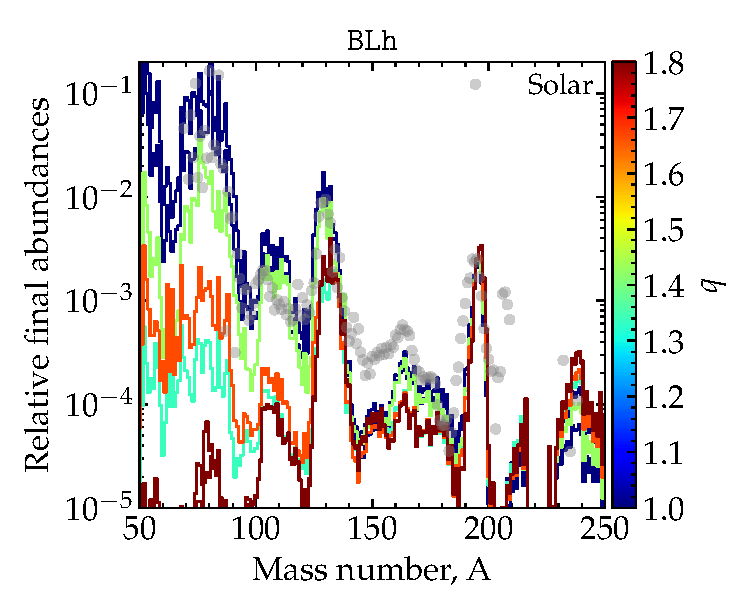
\includegraphics[width=0.45\textwidth]{nucleo/cc_nucleo_BLh_total.pdf}
    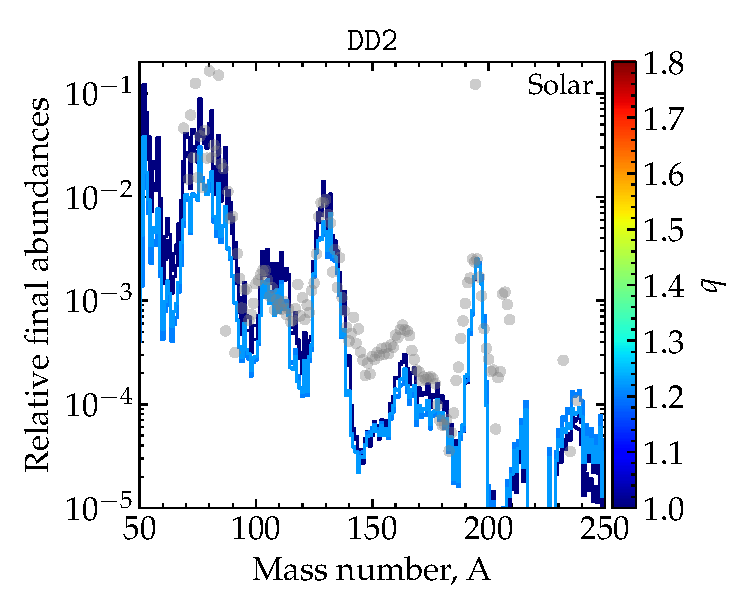
\includegraphics[width=0.45\textwidth]{nucleo/cc_nucleo_DD2_total.pdf}
    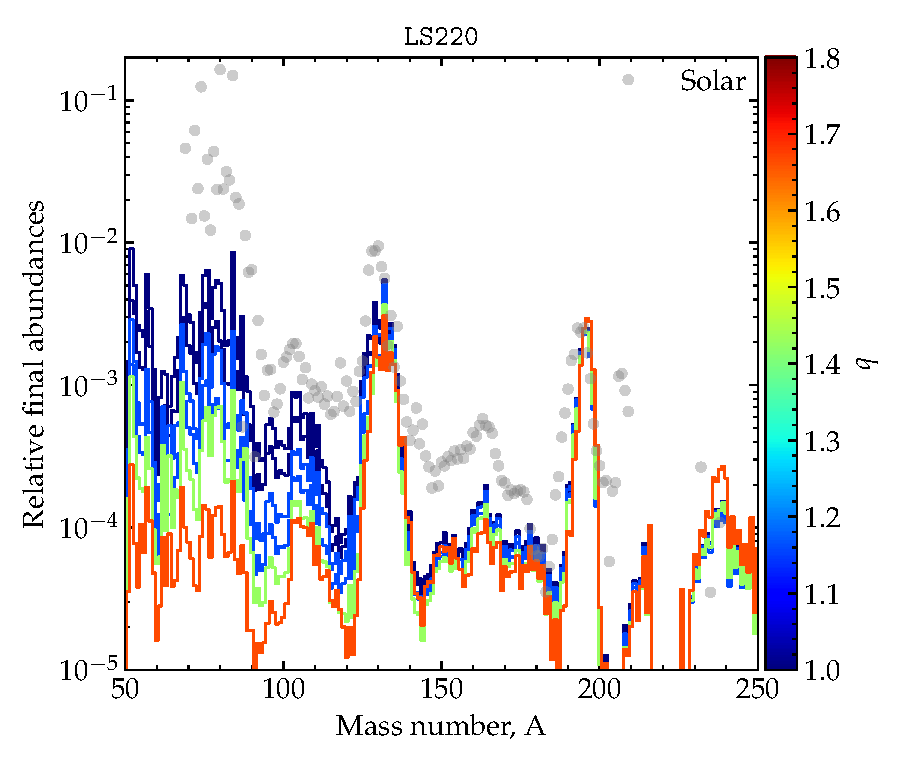
\includegraphics[width=0.45\textwidth]{nucleo/cc_nucleo_LS220_total.pdf}
    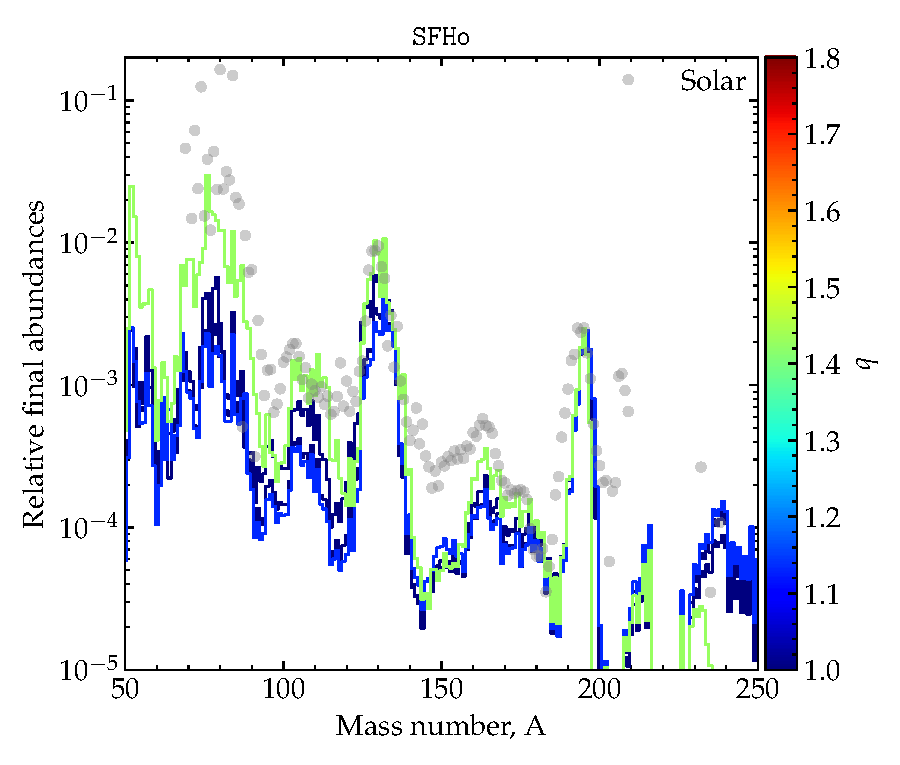
\includegraphics[width=0.45\textwidth]{nucleo/cc_nucleo_SFHo_total.pdf}
    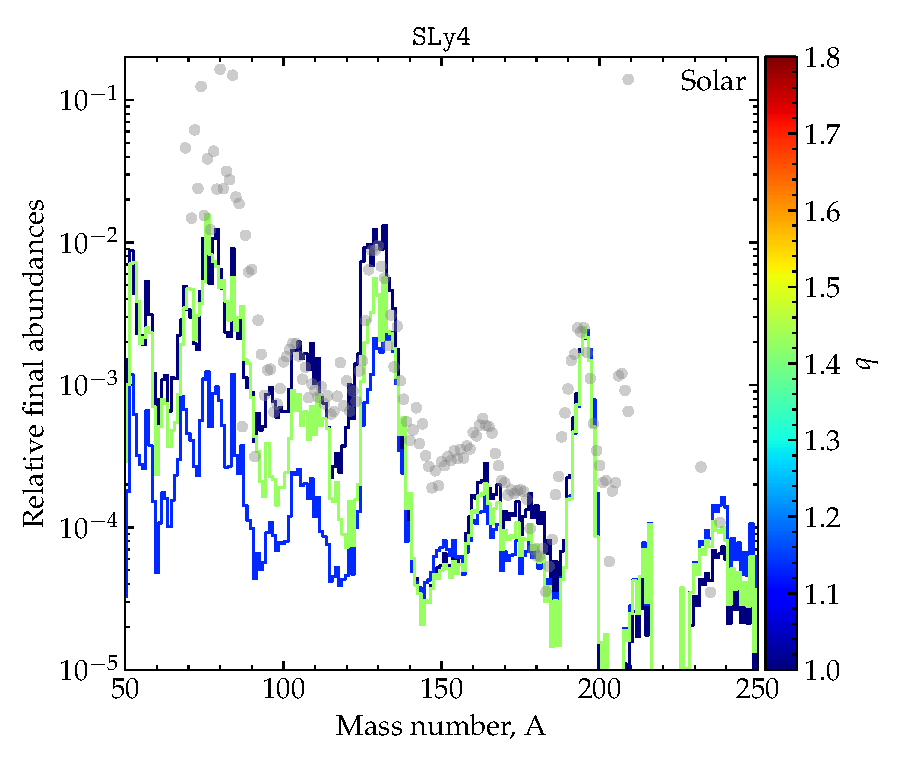
\includegraphics[width=0.45\textwidth]{nucleo/cc_nucleo_SLy4_total.pdf}
    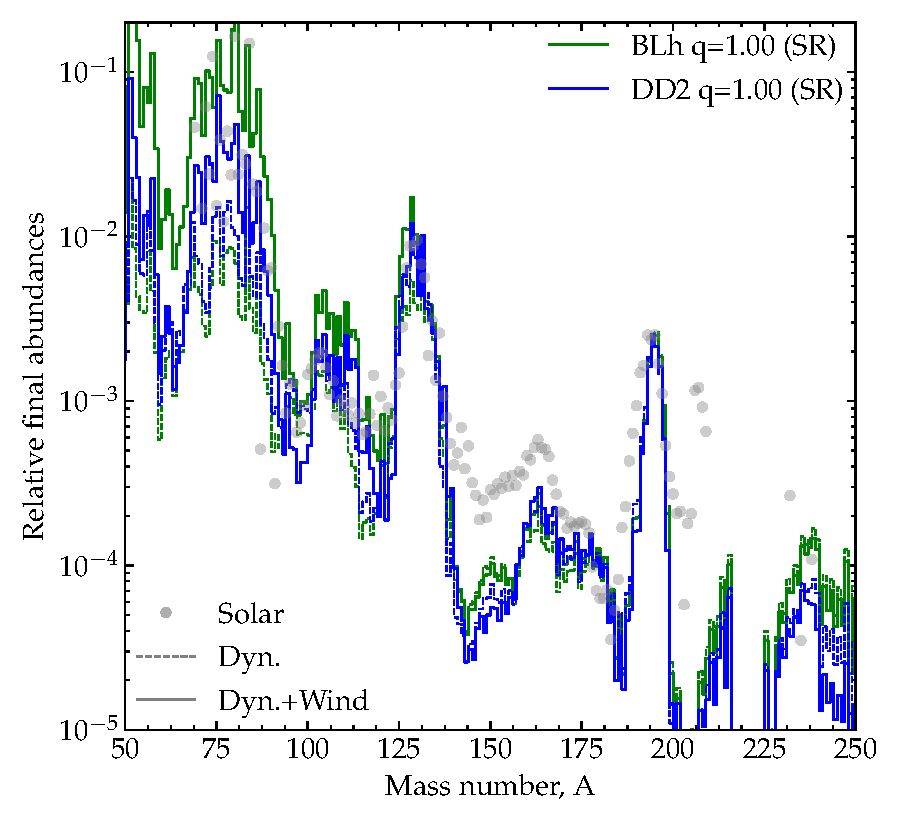
\includegraphics[width=0.42\textwidth]{nucleo/nucleo_dd2_blh.pdf}
    \caption{Nucleosynthesis yields for all simulations. Each %% panel
        of the first five panels 
        shows a different EOS and the scale color the dependency on the
        mass ratio. The nucleosynthesis is computed on the total ejecta
        computed during the simulations and 
        composed of the \ac{DE} (all models) plus the \ac{SWW} 
        (for the long-lived remnants listed in
        Tab.~\ref{tab:spiralwavewind}.).
        %
        The last (bottom-right) panel compares the nucleosynthesis in
        the \ac{DE} and \ac{SWW} for the long-lived
        remnants. The inclusion of the \ac{SWW} contributes to 
        improve the agreement with solar data for elements around the first peak.
        (Adapted from \citet{Nedora:2020pak})
    }
    \label{fig:nucle:totalyields}
\end{figure*}

The nucleosynthesis calculations are performed in postprocessing
following the same approach as in \cite{Radice:2016dwd,Radice:2018pdn}.

Here we briefly outline the procedure. 
Expanding ejecta undergoes the rapid neutrino capture nucleosynthesis, (\rproc{}).
In \citet{Lippuner:2015gwa} a new nuclear reaction network was presented 
(see Appendix~\ref{app:nuc} for more details). 
Using the parametrized \rproc{} calculations it is possible to map the ejecta 
parameters (discussed below) onto the final nucleosynthetic yields of our simulations.
The procedure is the following. 
For a given ejecta type (\eg, \ac{DE} or \ac{SWW}) we obtain the electron fraction,
entropy, velocity and rest mass density at a given extraction sphere 
(see Sec.\ref{sec:method:ejecta}).
The $r$-process in a given fluid element depends on how fast it decompresses from the 
merger environment (see Appendx~\ref{app:nuc}). 
This can be parametrized with the expansion timescale, $\tau$, assuming a specific 
velocity profile for the ejecta. We assume the homologous expansion \red{explain!}.
This assumption holds, as ejecta reaching the extraction sphere has already 
significantly decompressed and its density decreased ${\sim}3$~orders of magnitude. 
For the homologous expanding fluid, the density as a function of time reads 

\begin{equation}
    \rho(t) = \rho_E\Big(\frac{\upsilon_E t}{r_E}\Big)^{-3} = 
    \rho_E\Big(\frac{\upsilon_E t}{r_E}t\Big)^{-3},
    \label{eq:nuc:rho_homolog}
\end{equation}

where $\rho_E$ and $\upsilon_E$ are the density and velocity of the fluid element 
when it crosses the radius $r_E$. 
%% ---
The density in the nucleosynthesis calculations has the profile \citep{Lippuner:2015gwa} 

\begin{equation}
    \rho(t) = \rho(s, Y_e, T=6\text{GK})\Big(\frac{3\tau}{e t}\Big)^3
    \label{eq:nuc:rho_nuccalc}
\end{equation}

where $e$ is the Euler's number, and $s$ and $Y_e$ are the fluid entropy and 
electron fraction.

Solving together Eq.~\eqref{eq:nuc:rho_homolog} and Eq.~\eqref{eq:nuc:rho_nuccalc},
the expansion timescale $\tau$ can be extracted.

In order to compute the nucleosynthetic yields we bin the ejecta in the 
parameter space of $(s, Y_e, \tau)$. 
%% --- 
Under the assumption of homologous expansion the \rproc{} outcome depends on 
the these quantities and can be precomputed.
%% ---
We compute the total nucleosynthetic yields by summing the contributions from 
each bin.

%% -------------------------------------

%However, part of the uncertainty lies in the yet insufficient understanding of the nucleosynthetic yields from the neutron star mergers. Here we study the $r-$process
%abundances from the mergers, focusing on the effect of mass-ratio and equation of state. Complimentary to the previous study \cite{Radice:2018pdn}, we include the post-dynamical ejecta, \textit{e.g.,} \swind, where the lifetime of the remnant is sufficiently long. \\
%
%For the nucleosynthesis calculations we employ the same approach as in \cite{Radice:2016dwd} and \cite{Radice:2018pdn} which we outline briefly. Consider the outflowing material, crossing the coordiante sphere surface with $R\approx294$km that satisfies the criteria to be unbound, (geodesic for the dynamical ejecta and Bernoulli for the \swind) the following properties. WE extract its electron fraction n $Y_{e,R}$, specific entropy $s_R$, velocity $\upsilon_R$ and the rest-mass density $\rho_{0,R}$. In addition, we assume that the following expansion of the material is homologous, \textit{i.e.,}
%
%\begin{equation}
%\rho_{0}(t) = \rho_{0,R}\Big(\frac{\upsilon_R}{cR}t\Big)^{-3}.
%\label{eq:nucleo:rho_t}
%\end{equation}
%
%Then we match the density decrease with radius, with the $\rho$ behavior available in the parameterized $r$-process calculations of \cite{Lippuner:2015gwa}
%
%\begin{equation}
%\rho_{0}(t) = \rho_{0}(s, Y_e, T=6\text{GK})\Big(\frac{3\tau}{et}\Big)^3,
%\label{eq:nucleo:rho_t_lipp}
%\end{equation}
%
%where $\tau$ is the expansion timescale, and $e$ is the constant $e\approxeq 2.718$. Matching the equations \ref{eq:nucleo:rho_t} and \ref{eq:nucleo:rho_t_lipp} yields $\tau$ as
%
%\begin{equation}
%\tau_d = \frac{eR}{3\upsilon_R}\Bigg(\frac{\rho_R}{\rho_0}\Bigg)^{1/3}.
%\end{equation}
%
%Nucleosynthesis network calculations allow for a homologous expansion  to precompute the yields as a function of $\{\rho_{0,R},s_R,Y_{e,R},\tau_R\}$. Binning the corresponding ejecta parameter space, we can then use this precomputed data to gauge the nucleosynthetic yields in every bin of ejecta. Summing them, we obtain the total yield. For the discussion of the uncertainty of this method, see \cite{Radice:2018pdn}. \\
%
%It is also worth noting other approaches to nucleosynthesis computations in ejecta. In principle, the method should involve tracking numerous isotopic abundances of the material, that is moving along the fluid flow, undergoing fission, mixing and spallation, accounting for the EOS dependent feedback to the underlying flow. This however would require modifications to the composition equation and would make models computationally very expensive. A simplification to this approach would be to ignore the backreaction of nucleosynthesis to the flow dynamics, following the composition changes of Lagrangian traces advocated by it. It is believed that fission, while producing entropy that alters the burning in non-trivial way, amounts to only marginally changing the flow dynamics of lightly bound material \vn{it is however interesting to see how this would change the \swind mass}. Thus, the tracer approach is reasonable approximation, that is widely used. The technical difference with respect to the arropach employed in this work, is that the density history $\rho(t)$ is tracked in the ejecta instead of the assumption of homologous expansion. The entropy $s_0$ and electron fraction $Y_{e,0}$ are extracted at the time $t_0$ and then evolved using a self-heating nuclear reaction network \cite{Freiburghaus:1999}. \\
%
%The comparison between tracer method and homologous expansion one is performed in \cite{Radice:2018pdn}. It was concluded that within a factor of two, methods yield similar results. However, several caveats were pointed out with respect to the errors arising in ignoring the actual density history ($25\%$). On the other had it was stated that due to the approximation of Eualian flow with Lagrangian the error of $\sim 40\%$ can be expected. \\
%
%Here, employing the homologous expansions method. We report the relative abundances of different isotopes synthesized by the $r$-process \red{32} years \vn{not sure where this number is set up} after the merger in the material ejected from the system. In the \textit{short-lived} cases this encompasses only the dynamical ejecta, while in the \textit{long-lived} ones (see table \ref{tab:wind}) it includes the \swind. As the electron fraction is the most important quantity determining the outcome of the $r$-process \cite{Lippuner:2015gwa,Radice:2016dwd}, we report it for selected \textit{long-lived} models in figure \ref{fig:ejecta:bern:hist}. In the figure \ref{fig:nucleo:dynvswind} we compare how the inclusion of the \swind changes the abundances of two representative models and in the figures \ref{fig:nucleo:dynonly} and \ref{fig:nucleo:dynvswind} we show the total abundances of a large  subset of models, investigating the effect of mass ration and EOS (without and with the inclusion of \swind respectively). In all cases, we compare our abundances with the up-to-date solar ones from \cite{Prantzos2020} (for a review of the solar system abundances see \textit{e.g.,} \cite{Pritychenko:2019xvf}). The latter are normalized to the sum of all elements, while the model abundances are normalized to the solar at $A=195$. This is justified as long as ejecta contains very neutron rich material, as the nuclear fission cycling leads to a robust profile that follows the third $r$-process peak \cite{Lippuner:2015gwa}.\\
%
%The \cite{Radice:2018pdn} presents the systematics of the nucleosynthetic yields of a large subset of models, for which neutrino re-absorption has been neglected. Here we extent this by performing a similar analysis albeit with the subset of models that include the neutrino re-absorption. In addition, the subgrid turbulence is included in most of our models. However, its effect is much weaker then the one of the mass-ratio. Indeed, the figure \ref{fig:nucleo:dynonly} shows a model's ability to reproduce the solar $1$st and $2$nd r-process peaks, at $A\sim 100$ and $A\sim 125$ respectively strongly depended on the mass-ratio. Higher $q$ models, whose dynamical ejecta is mostly of tidal tail origin with very low electron fraction show severe underproduction of light $r$-process material, while $q=1$ DD2 and BLh models are able to reproduce both peaks reasonably well. This is the result of inclusion of neutrino reabsortion as it increases the $Y_e$ of the shocked component of the ejecta \cite{Radice:2018pdn}. Note, however, that in \cite{Papenfort:2018bjk} the effect of $q$ was not found. But similar to both studies, with respect to the equation of state, we do not observe consistent changes between still anf soft ones. This has also been the case in the aforementioned study.\\
%
%Important to note the actinides production, elements with atomic number $A\sim 230$. It was previously reported that in binary neutron star merger ejecta these materiel is overproduced (see \textit{e.g.,} \cite{Giuliani:2019oot}). However, we hint that this conclusion might partially be motivated by a choice of normalization. If we employ the physically motivated normalization to $A = 195$ of solar abundances, we observe that the actinides abundances are consistent with solar. We also note that there is dependency on the mass-ratio, motivated once again, by the ejecta composition. The very low $Y_e$ of highly assymetric models leads to significant boost in actinides production. This is the case for $q=1.8$ of BLh and $q=1.67$ of LS220. \\
%
%Indeed, to explain the $^{232}$Th solar abundances the average electron fraction in the ejecta should lower and any of our models except promptly collapsing ones can achieve. This underlines the importance of such mergers for $r$-process nucleosynthesis. We however emphases, that with adopted in this work normalisation, we do not observe overproduction of actinides, that was reported in \cite{Holmbeck:2019xnd}. \\
%
%+
%In the \textit{long-lived} case, the dynamical ejecta amounts to a small fraction of the total mass of material leaving the system. The second, more massive component, is the \swind. Its overall high electron fraction (see Fig. \ref{fig:ejecta:bern:hist}) implies that the weak $r$-process is dominant one here and light elements $A<195$ are primarily produced. In figure \ref{fig:nucleo:dynvswind} we compare the relative abundances from nucleosynthesis in dynamical ejecta only, with the total ones. Owing to the normalization to the $3$rd peak, it is reproduced in both cases, and the important difference lies in the $1$st and $2$nd peaks. In case of BLh we see that solar abundances of even very light elements $A\sim75$ are robustly reproduced. However there is an overproduction of $A\sim 110$ and $A\sim 130$ elements. The DD2 model, on the other hand, shows an overall lower total abundances. This is attributed to the slightly lower average electron fraction in DD2 (Fig. \ref{fig:ejecta:bern:hist}) while the ejecta masses are very similar (Fig.\ref{fig:mej:bern}). \\
%
%In the figure \ref{fig:nucle:totalyields} we investigate the total mass-ratio dependence of the total abundances. It is important to emphasis that in \textit{short-lived} cases this is the abundances of the dynamical ejecta only. Thus we limit this discussion to the DD2 and BLh models, most of which are sufficiently long with only extreme high $q$ BLh ones being an exception. Notably, the abundances strong $q$ dependence observed in dynamical ejecta, is not present for total ejecta, and all the $r$-process peaks are reasonably well reproduced by all the \textit{long-lived} models. This is not too surprising owing to the robust properties of the \swind, that change only marginally between different models. \\
%
%Overall, we find that dynamical ejecta of asymmetric models in general underproduces the $1$st and $2$nd r-process peaks due to its low average electron fraction. Equal mass DD2 and BLh models however are able to reproduce these peaks. Meanwhile, the total ejecta of DD2 and $q<1.7$ BLh models reproduces both, $1$st and $2$nd r-process peaks reasonably well irrespective of the mass-ratio, showing that the complete solar $r$-process abundances can be recovered if the remnant is \textit{long-lived}. This further supports the hypothesis, that binary netuton stars are the prime source of $r$-process material in the Universe.\\
%
%It is however, important to note that nucleosynthetic yields are subjected to the choice of nuclear input data. In particular, the choice of fission fragment distributions and neutron induced fission rates may have a large impact on abundances in the region of the $1$st and $2$nd peaks \cite{Eichler:2014kma}. The symmetric fission fragment distributions used in our calculations does most likely underproduce material in this region. In addition, as the neutrino-matter interaction rates roughly scale with the square of the incoming neutrino energy. Thus, the nucleosynthetic yields depend on the details of the neutrino radiation spectra \cite{Foucart:2016rxm}. The energy integrated scheme, employed in this work, does not allow us to take this effect into account (see, however, \cite{Radice:2018pdn} where different neutrino energy distributions were studied). It was recently pointed out that the neutrino resonant oscillations and fast flavor conversion might occur in NS merger remnants \cite{Zhu:2016mwa,Frensel:2016fge,Deaton:2018ser}. This might modify the nucleosynthesis of light $r$-process elements \cite{Wu:2016pnw}. Thus there is a need for more sophisticated simulations with spectral neutrino transport taking into account the neutrino oscillations. \\
%
%In addition to the dynamical ejecta and \swind, the $r$-process nucleosynthesis occurs in the secular ejecta. In particular in neutrino-driven winds, where neutrino irradiation of the expanding ejecta considerably increases the electron fraction. If the velocity of the ejecta sufficiently low, the material achieves $Y_e$ given by the weak equilibrium in optically thin conditions with neutrinos \cite{Qian:1996xt}. During the early post merger phase this $(Y_e)_{eq}\leq 0.45$ which allows for a weak $r$-process nucleosynthesis of light elements $A<130$ to occur \cite{Dessart:2008zd,Perego:2014fma,Foucart:2016rxm,Martin:2015hxa}. In addition, is expected that the dominant source of ejecta from the merger is the viscously-driven outflow from massive disk, if it forms after the merger. Properties on such outflow has been recently investigated in a framework of axisymmetric BH-torus systems \cite{Fernandez:2013tya,Just:2015fda}. The $Y_e$ distribution was found to be broad allowing all $r$-process elements from the $1$st to the $3$rd peak, as well actinides, to be synthesized in proportions close to solar (\textit{e.g.,} \cite{Wu:2016pnw}). If the \textit{long-lived} remnant is present however, the properties of the viscous ejecta are expected to be significantly altered by the large amount of neutrinos emitted over the diffusion time scale (seconds, \textit{e.g.,} \cite{Dessart:2008zd,Perego:2017fho}). 



%% -------------------------------------



\red{Radice:2018pdn disussion on the accuracy/}.

\red{Something to check}
\gray{
    We do not nd material with expansion timescale of
    less than 0:5 ms. This seems to exclude the neutron freezeout
    scenario proposed by Metzger et al. (2015). However,
    the lack of a very fast component of the ejecta might also
    be due to numerical effects. Our resolution is probably not
    high enough to track the very small fraction of the ejecta
    expected to experience neutron freeze-out in the scenario
    proposed by Metzger et al. (2015).
}


%% ----------- results ----------------- 

With the procedure outlined above we compute the isotopic abundances of 
the \rproc{} elements $32$~years after merger. 
%% ---
The novelty of the results presented in this section is in the more 
advanced neutrino treatment, as all out models include the effects of neutrino 
self absorption (in comparison with \citet{Radice:2018pdn}), the inclusion 
of the \ac{SWW}, and models with high \mr{}, $q\geq1.8$. 
%% ---

In the Fig.~\ref{fig:nucle:totalyields} (except the bottom right panel), 
we show the nucleosynthesis yields from overall ejecta with each panel 
containing all models fro a given \ac{EOS}, with the \mr{} being color-coded.
For models with short-lived \ac{MNS} remnants the total ejecta is compised 
of the \ac{DE} only, while for models with long-lived ones, the total ejeta 
consists of \ac{DE} and \ac{SWW}. 
%% --- 
We compare the model abundances with the recently updated solar residual 
\rproc{} abundances from \citet{Prantzos2020} 
(for a review of the solar system abundances see \eg~\citet{Pritychenko:2019xvf}).
For the qualitative comparison between models and observations we employ 
the following normalization. 
The model abundances are multiples by a constant factor that makes the abundances at 
$A=195$ equal solar.
%% --- 
From the plot we observe that final \rproc{} abundances in the ejecta from models that 
form long-lived \ac{MNS} remnants with DD2 and BLh \acp{EOS}, are in a greement with 
solar across all three \rproc{} peaks. 
\red{add some info on peaks themselves.}
Due its robust properties, the \ac{SWW} allows for the complete reproduction 
of the solar \rproc{} abundances. 
\red{A note on the high Ye and light element productioN?}
%% --- 
With respect to the models with short-lived remnants, the final \rproc{} eject abundances 
at solar $1$st and $2$nd \rproc{} peaks, (at $A\sim 75$ and $A\sim 125$ respectively) 
depend strongly on \mr{}. 
For instance, models with high \mr{} have \ac{DE} of tidal origin mostly with low 
electron fraction. The final \rproc{} abundances in this ejecta show the underproduction 
of light elements. 
The final abundances in ejecta from equal mass binaries, 
however, shows that even light \rproc{} elements are 
synthesized. This is because the neutrino reabsorption raises the electron fraction 
in the shocked component of the \ac{DE} \citep{Wanajo:2014wha,Radice:2018pdn}. 

%% --- 
We observed that final abundances in the ejecta in all our models show the 
presence of actinides, elements with $A\sim230$. 
The amount of actinides produced, however, depends strongly on the ejecta 
electron fraction, and thus, on the binary \mr{}.
The agreement with solar abundances is found only for very asymmetric binaries. 
Notably, that only for the binaries with the highest \mr{}, $q\sim1.8$, the 
\rproc{} in the \ac{DE} results in both $3$rd peak and actinides(at $^{232}$Th) abundances 
close to solar values. 
This suggests that the high \mr{} mergers or \ac{NSBH} mergers might be an 
important contributor to the cosmic chemical evolution.

%%--- Bottom right panel
The total ejecta from the models with long-lived \ac{MNS} remnants is dominated by
the \ac{SWW}, as its mass is generally limited by the \ac{MNS} lifetime 
or by the evolved time (Sec.~\ref{sec:results:ejecta:sww})
In the bottom-right panel of Fig.~\ref{fig:nucle:totalyields} we show separately the 
final abundances from the \rproc{} in the \ac{DE} and in the \ac{DE} plus \ac{SWW}. 
The electron fraction of the \ac{SWW} is higher than that of the \ac{DE} 
(see Fig. \ref{fig:ejecta:bern:hist}), and this the \rproc{} nucleosynthesis in the 
\ac{SWW} produces primarily light elements around the first \rproc{} peak, $A<95$.
We recall here, that due to the choice of the normalization, all abundances are up-scaled 
to reproduce the $A=195$ peak. We asses here the relative abundances at $1$st and $2$nd
\rproc{} peaks.
%% ---
The plot shows that for the BLh models the amount of lighter elements, $A\sim75$, is higher with 
respect to the DD2 model. This can be attributed to the higher electron fraction in the 
\ac{SWW} of the former (see Fig. \ref{fig:ejecta:bern:hist}).
In both cases, however, the abundances of light elements are very close to slolar 
\red{can be extended by adding plot from the Letter}

%% --- other ejecta types
The \rproc{} is expected to take place in other types of ejecta from \ac{BNS} mergers.
In \nwind{} the neutrino irradiation raises the electron fraction, that, depending 
on the ejecta velocity, can reach the $Y_e\leq 0.45$ \citep{Qian:1996xt}. 
At this pint the weak equilibrium sets in between the ejecta and neutrinos.
High electron fraction implies that only the light elements will be produced.
The numerical studies indeed support this picture 
\citep{Dessart:2008zd,Perego:2014fma,Just:2014fka,Martin:2015hxa,Foucart:2016rxm}. 
%% ---
The bulk of the ejecta from \ac{BNS} mergers is expected to come in the form of 
viscous- and recombination-driven winds, This ejecta, however, is expected to take 
place over the longer timescales than those of our simulations.
Studies have shown that this ejecta has a broad distribution of the electron fraction 
and the \rproc{} nucleosynthesis within it would produce light as well as heavy elements
\citep{Fernandez:2013tya,Just:2014fka,Wu:2016pnw,Siegel:2017nub,Fujibayashi:2017puw,Fernandez:2018kax}.
The production of the heavy \rproc{} elements, however, might be supressed in this winds
if the long-lived \ac{MNS} is present \citep{Metzger:2014ila,Lippuner:2017bfm}.